\documentclass[
    a4paper, 				% Page size
    fontsize=11pt, 			% Base font size
    twoside=true, 			% Use different layouts for even and odd pages (in particular, if twoside=true, the margin column will be always on the outside)
	%open=any, 				% If twoside=true, uncomment this to force new chapters to start on any page, not only on right (odd) pages
	%chapterentrydots=true, % Uncomment to output dots from the chapter name to the page number in the table of contents
	numbers=noenddot, 		% Comment to output dots after chapter numbers; the most common values for this option are: enddot, noenddot and auto (see the KOMAScript documentation for an in-depth explanation)
	fontmethod=modern, 		% Can also use "modern" with XeLaTeX or LuaTex; "tex" is the default for PdfLaTex, and "modern" is the default for those two.
	BCOR=10mm,				% Binding Correction, i.e. how much of the page is lost in the middle (0mm for spiral)
]{kaobook}

% Load my own additions
\usepackage[
	language=english,
	debug=false
]{ethesis}

\usepackage{blindtext} 					% Print text without any meaning for testing purposes
\usepackage[style=ieee]{kaobiblio}  				% Load special bib packages
\addbibresource{thesis.bib} 			% Bibliography file
\usepackage[framed=true]{kaotheorems}	% Load special math packages, incl. theorem envs
\usepackage{kaorefs}  					% Load special hyperref packages

\makeindex[columns=3, title=Alphabetical Index, intoc] % Make LaTeX produce the files required to compile the index
\makeglossaries % Make LaTeX produce the files required to compile the glossary
\import{./}{glossary.tex} % Include the glossary definitions
\makenomenclature{} % Make LaTeX produce the files required to compile the nomenclature

% Reset sidenote counter at chapters
%\counterwithin*{sidenote}{chapter}

%----------------------------------------------------------------------------------------

\begin{document}

%----------------------------------------------------------------------------------------
%	THESIS INFORMATION
%----------------------------------------------------------------------------------------

\title{Building a \qty{25}{\mega\hertz} NMR Spectrometer}
\subtitle{}
\logo{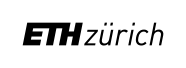
\includegraphics[width=4cm]{ethlogo}}
\author{Maximilian Stabel}
\born{03.11.1995}
\citizen{Germany}
\date{\today}

\examiner{Prof.\ Roland Riek\\Prof.\ Sebastian Kozerke}
\supervisor{Dr.\ Takuya Segawa}

\degree{Master of Science ETH in Electrical Engineering and Information Technology}
\shortdegree{MSc ETH EEIT}
\idnumber{20\=/954\=/590}  % Student ID

%----------------------------------------------------------------------------------------

\frontmatter % Denotes the start of the pre-document content, uses roman numerals

%----------------------------------------------------------------------------------------
%	COLOPHON
%----------------------------------------------------------------------------------------

\lowertitleback{
	\hypersetup{hidelinks}
	\color{blankcolor}
	\footnotesize

	\begin{tblr}{@{}rX[l]@{}}
		Name                                                    & \texttt{\textbf{\jobname{}}}                                                                                                      \\
		Compiled on                                             & \textbf{\DTMnow{}}                                                                                                                \\
		\faIcon{git-alt}                                        & \texttt{\textbf{\GitShortSHA{}} (\GitRefName{})}                                                                                  \\
		Engine                                                  & \prettybanner{}                                                                                                                   \\
		\href{https://www.latex-project.org/}{\LaTeX{} Version} & \hologo{\fmtname} (\fmtversion)                                                                                                   \\
		\glossaryname{}                                         & \texttt{makeglossaries}                                                                                                           \\
		\bibname{}                                              & biblatex + \hologo{biber}                                                                                                         \\
		Generator                                               & \texttt{latexmk}                                                                                                                  \\
		Class                                                   & \href{https://sourceforge.net/projects/koma-script/}{\KOMAScriptVersion{}} + \href{https://github.com/fmarotta/kaobook/}{kaobook} \\
		Font                                                    & \textrm{\showfont}, \textsf{Sans:\ \showfont}, \texttt{Mono:\ \showfont}                                                          \\
		Math Font                                               & \mathfont, Operators:\ \mathoperatorfont                                                                                          \\
		Font Size                                               & \normalfontsize{}pt                                                                                                               \\
	\end{tblr}%
}

%----------------------------------------------------------------------------------------
%	DEDICATION
%----------------------------------------------------------------------------------------

\dedication{
	\textit{%
		I may not have gone where I intended to go,\\
		but I think I have ended up where I needed to be.\\
	}%
	--- Douglas Adams
}

%----------------------------------------------------------------------------------------
%	OUTPUT TITLE PAGE AND PREVIOUS
%----------------------------------------------------------------------------------------

% Includes colophon, dedication, ...
\maketitle

%----------------------------------------------------------------------------------------
%	PREFACE
%----------------------------------------------------------------------------------------

\import{chapters/}{abstract.tex}%
\index{abstract}

%----------------------------------------------------------------------------------------
%	TABLE OF CONTENTS & LIST OF FIGURES/TABLES
%----------------------------------------------------------------------------------------

\begingroup % Local scope for the following commands

% Define the style for the TOC, LOF, and LOT
%\setstretch{1} % Uncomment to modify line spacing in the ToC
%\hypersetup{linkcolor=blue} % Uncomment to set the colour of links in the ToC
\setlength{\textheight}{230\hscale} % Manually adjust the height of the ToC pages

% Turn on compatibility mode for the etoc package
\etocstandarddisplaystyle % "toc display" as if etoc was not loaded
\etocstandardlines % "toc lines as if etoc was not loaded

\tableofcontents % Output the table of contents

\listoffigures % Output the list of figures

% Comment both of the following lines to have the LOF and the LOT on 
% different pages
\let\cleardoublepage\bigskip
\let\clearpage\bigskip

\listoftables % Output the list of tables

\listoflstlistings % Output the list of listings

\endgroup

%----------------------------------------------------------------------------------------
%	MAIN BODY
%----------------------------------------------------------------------------------------

\mainmatter{} % Denotes the start of the main document content, resets page numbering and uses arabic numbers
\setchapterstyle{kao} % Choose the default chapter heading style

\import{chapters/}{introduction.tex}
\import{chapters/}{background.tex}
\import{chapters/}{methods.tex}
\import{chapters/}{results-discussion.tex}
\import{chapters/}{conclusion.tex}

\appendix % From here onwards, chapters are numbered with letters, as is the appendix convention

\pagelayout{wide} % No margins
\addpart{Appendix}
\pagelayout{margin} % Restore margins

\import{chapters/}{appendix.tex}

%%% KAO stuff - Remove later!
\import{chapters/kao/}{introduction.tex}
\pagelayout{wide} % No margins
\addpart{Class Options, Commands and Environments}
\pagelayout{margin} % Restore margins

\import{chapters/kao/}{options.tex}
\import{chapters/kao/}{textnotes.tex}
\import{chapters/kao/}{figsntabs.tex}
\import{chapters/kao/}{references.tex}

\pagelayout{wide} % No margins
\addpart{Design and Additional Features}
\pagelayout{margin} % Restore margins

\import{chapters/kao/}{layout.tex}
\import{chapters/kao/}{mathematics.tex}

\appendix % From here onwards, chapters are numbered with letters, as is the appendix convention

\pagelayout{wide} % No margins
\addpart{Appendix}
\pagelayout{margin} % Restore margins

\import{chapters/kao/}{appendix.tex}

\pagelayout{wide}
\setchapterstyle{kao}
\chapter{Test}
\blindtext{}

%----------------------------------------------------------------------------------------

\backmatter % Denotes the end of the main document content
\setchapterstyle{plain} % Output plain chapters from this point onwards

%----------------------------------------------------------------------------------------
%	BIBLIOGRAPHY
%----------------------------------------------------------------------------------------

% The bibliography needs to be compiled with biber using your LaTeX editor, or on the command line with 'biber main' from the template directory

\defbibnote{bibnote}{References in citation order.\par\bigskip} % Prepend this text to the bibliography
\printbibliography[heading=bibintoc, title=Bibliography, prenote=bibnote] % Add the bibliography heading to the ToC, set the title of the bibliography and output the bibliography note

%----------------------------------------------------------------------------------------
%	NOMENCLATURE
%----------------------------------------------------------------------------------------

% The nomenclature needs to be compiled on the command line with 'makeindex main.nlo -s nomencl.ist -o main.nls' from the template directory

\nomenclature{$c$}{Speed of light in a vacuum inertial frame}
\nomenclature{$h$}{Planck constant}

\renewcommand{\nomname}{Notation} % Rename the default 'Nomenclature'
\renewcommand{\nompreamble}{The next list describes several symbols that will be later used within the body of the document.} % Prepend this text to the nomenclature

\printnomenclature % Output the nomenclature

%----------------------------------------------------------------------------------------
%	GREEK ALPHABET
% 	Originally from https://gitlab.com/jim.hefferon/linear-algebra
%----------------------------------------------------------------------------------------

\vspace{1cm}

{\usekomafont{chapter}Greek Letters with Pronunciations} \\[2ex]
\begin{center}
	\newcommand{\pronounced}[1]{\hspace*{.2em}\small\textit{#1}}
	\begin{tabular}{l l @{\hspace*{3em}} l l}
		\toprule
		Character            & Name                            & Character              & Name                                   \\
		\midrule
		$\alpha$             & alpha \pronounced{AL-fuh}       & $\nu$                  & nu \pronounced{NEW}                    \\
		$\beta$              & beta \pronounced{BAY-tuh}       & $\xi$, $\Xi$           & xi \pronounced{KSIGH}                  \\
		$\gamma$, $\Gamma$   & gamma \pronounced{GAM-muh}      & o                      & omicron \pronounced{OM-uh-CRON}        \\
		$\delta$, $\Delta$   & delta \pronounced{DEL-tuh}      & $\pi$, $\Pi$           & pi \pronounced{PIE}                    \\
		$\epsilon$           & epsilon \pronounced{EP-suh-lon} & $\rho$                 & rho \pronounced{ROW}                   \\
		$\zeta$              & zeta \pronounced{ZAY-tuh}       & $\sigma$, $\Sigma$     & sigma \pronounced{SIG-muh}             \\
		$\eta$               & eta \pronounced{AY-tuh}         & $\tau$                 & tau \pronounced{TOW (as in cow)}       \\
		$\theta$, $\Theta$   & theta \pronounced{THAY-tuh}     & $\upsilon$, $\Upsilon$ & upsilon \pronounced{OOP-suh-LON}       \\
		$\iota$              & iota \pronounced{eye-OH-tuh}    & $\phi$, $\Phi$         & phi \pronounced{FEE, or FI (as in hi)} \\
		$\kappa$             & kappa \pronounced{KAP-uh}       & $\chi$                 & chi \pronounced{KI (as in hi)}         \\
		$\lambda$, $\Lambda$ & lambda \pronounced{LAM-duh}     & $\psi$, $\Psi$         & psi \pronounced{SIGH, or PSIGH}        \\
		$\mu$                & mu \pronounced{MEW}             & $\omega$, $\Omega$     & omega \pronounced{oh-MAY-guh}          \\
		\bottomrule
	\end{tabular} \\[1.5ex]
	Capitals shown are the ones that differ from Roman capitals.
\end{center}

%----------------------------------------------------------------------------------------
%	GLOSSARY
%----------------------------------------------------------------------------------------

% The glossary needs to be compiled on the command line with 'makeglossaries main' from the template directory

\setglossarystyle{listgroup} % Set the style of the glossary (see https://en.wikibooks.org/wiki/LaTeX/Glossary for a reference)
\printglossary[title=Special Terms, toctitle=List of Terms] % Output the glossary, 'title' is the chapter heading for the glossary, toctitle is the table of contents heading

%----------------------------------------------------------------------------------------
%	INDEX
%----------------------------------------------------------------------------------------

% The index needs to be compiled on the command line with 'makeindex main' from the template directory

\printindex % Output the index

%----------------------------------------------------------------------------------------
%	Declaration of Originality
%----------------------------------------------------------------------------------------

\cleardoubleoddpage{}

\chapter{Declaration of originality}

I hereby confirm that I am the sole author of the written work here enclosed and that I have compiled it in my own words. Parts excepted are corrections of form and content by the supervisor.

\vfill

\makeatletter
\begin{center}
	\begin{tabular}[t]{@{}ll@{}}%
		\textbf{Title of work}: & \@title  \\
		\textbf{Authored by}:   & \@author \\
	\end{tabular}
\end{center}
\makeatother

\vfill

With my signature, I confirm that
\begin{itemize}
	\item I have committed none of the forms of plagiarism described in the \enquote{\href{https://www.ethz.ch/content/dam/ethz/main/education/rechtliches-abschluesse/leistungskontrollen/plagiarism-citationetiquette.pdf}{Citation~etiquette}} information sheet.
	\item I have documented all methods, data and processes truthfully.
	\item I have not manipulated any data.
	\item I have mentioned all persons who were significant facilitators of the work.
\end{itemize}

I am aware that the work may be screened electronically for plagiarism.

\signaturefield{}

%----------------------------------------------------------------------------------------

\end{document}
